%%%% Better Poster latex template example v1.0 (2019/04/04)
%%%% GNU General Public License v3.0
%%%% Rafael Bailo
%%%% https://github.com/rafaelbailo/betterposter-latex-template
%%%% 
%%%% Original design from Mike Morrison
%%%% https://twitter.com/mikemorrison

\documentclass[a0paper,fleqn]{betterposter}

%%%% Uncomment the following commands to customise the format

%% Setting the width of columns
% Left column
%\setlength{\leftbarwidth}{0.25\paperwidth}
% Right column
%\setlength{\rightbarwidth}{0.25\paperwidth}

%% Setting the column margins
% Horizontal margin
%\setlength{\columnmarginvertical}{0.05\paperheight}
% Vertical margin
%\setlength{\columnmarginhorizontal}{0.05\paperheight}
% Horizontal margin for the main column
%\setlength{\maincolumnmarginvertical}{0.15\paperheight}
% Vertical margin for the main column
%\setlength{\maincolumnmarginhorizontal}{0.15\paperheight}

%% Changing font sizes
% Text font
%\renewcommand{\fontsizestandard}{\fontsize{28}{35} \selectfont}
% Main column font
%\renewcommand{\fontsizemain}{\fontsize{28}{35} \selectfont}
% Title font
%\renewcommand{\fontsizetitle}{\fontsize{28}{35} \selectfont}
% Author font
%\renewcommand{\fontsizeauthor}{\fontsize{28}{35} \selectfont}
% Section font
%\renewcommand{\fontsizesection}{\fontsize{28}{35} \selectfont}

%% Changing font sizes for a specific text segment
% Place the text inside brackets:
% {\fontsize{28}{35} \selectfont Your text goes here}

%% Changing colours
% Background of side columns
%\renewcommand{\columnbackgroundcolor}{black}
% Font of side columns
%\renewcommand{\columnfontcolor}{gray}
% Background of main column
%\renewcommand{\maincolumnbackgroundcolor}{empirical}
%\renewcommand{\maincolumnbackgroundcolor}{theory}
%\renewcommand{\maincolumnbackgroundcolor}{methods}
%\renewcommand{\maincolumnbackgroundcolor}{intervention}
% Font of main column
%\renewcommand{\maincolumnfontcolor}{gray}

\begin{document}	
\betterposter{
%%%%%%%% MAIN COLUMN

\maincolumn{
%%%% Main space

\textbf{Main finding} goes here,
\\translated into \textbf{plain English}.
\\\textbf{Emphasize} the important words.
}{
%%%% Bottom space

%% QR code
\qrcode{img/qrcode}{img/smartphoneWhite}{
\textbf{Take a picture} to
\\download the full paper
}
% Smartphone icon
% Author: Freepik
% Retrieved from: https://www.flaticon.com/free-icon/smartphone_65680

%% Compact QR code (comment the previous command and uncomment this one to switch)
%\compactqrcode{img/qrcode}{
%\textbf{Take a picture} to
%\\download the full paper
%}

}

}{
%%%%%%%% LEFT COLUMN

\title{Parallelization in R}
\author{Sven Nekula}
\author{Joshua Simon}
\author{Eva Wolf}
\institution{Optional Institution Under Name}

\section{Introduction}
Here is an itemised list:
\begin{itemize}
\item The first item.
\item The second item.
\item The third item.
\end{itemize}

\section{A Diagram}
Here is a diagram:
\begin{center}
% Linear regression
% Author: Henri Menke
% Retrieved from: http://www.texample.net/tikz/examples/linear-regression/
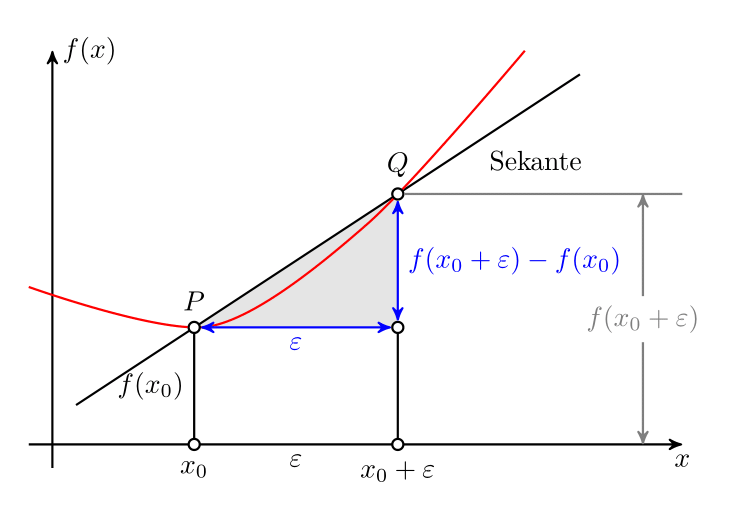
\includegraphics[width=\textwidth]{img/tikzexample1}
\end{center}

\section{Fundamental Theorem\\of Calculus}
If $f$ is continuous on the closed interval $[a,b]$ and $F$ is the indefinite integral of $f$ on $[a,b]$, then
\begin{equation}
\int_a^b f(x)\,\mathrm{d}x = F(b)-F(a).
\end{equation}

\section{Conclusion}
This is a great poster format!

%% This fills the space between the content and the logo
\vfill

%% Institution logo

\includegraphics[width=\textwidth]{img/logo}\\

}{
%%%%%%%% RIGHT COLUMN

Here you can add \textbf{supplementary material}. For instance, a new diagram:
\begin{center}
% Commutative diagram with edges passing under/over
% Author: Stefan Kottwitz, http://texblog.net/
% Retrieved from: http://www.texample.net/tikz/examples/commutative-diagram/
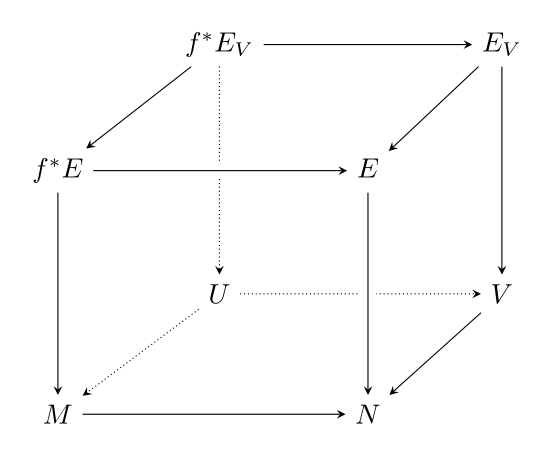
\includegraphics[width=\textwidth]{img/tikzexample2}
\end{center}

Some cute ducklings:
\begin{center}
% Picture of ducklings
% Author: Magda Ehlers, https://www.pexels.com/@magda-ehlers-pexels
% Retrieved from: https://www.pexels.com/photo/selective-focus-photo-of-flock-of-ducklings-perching-on-gray-concrete-pavement-1300355/
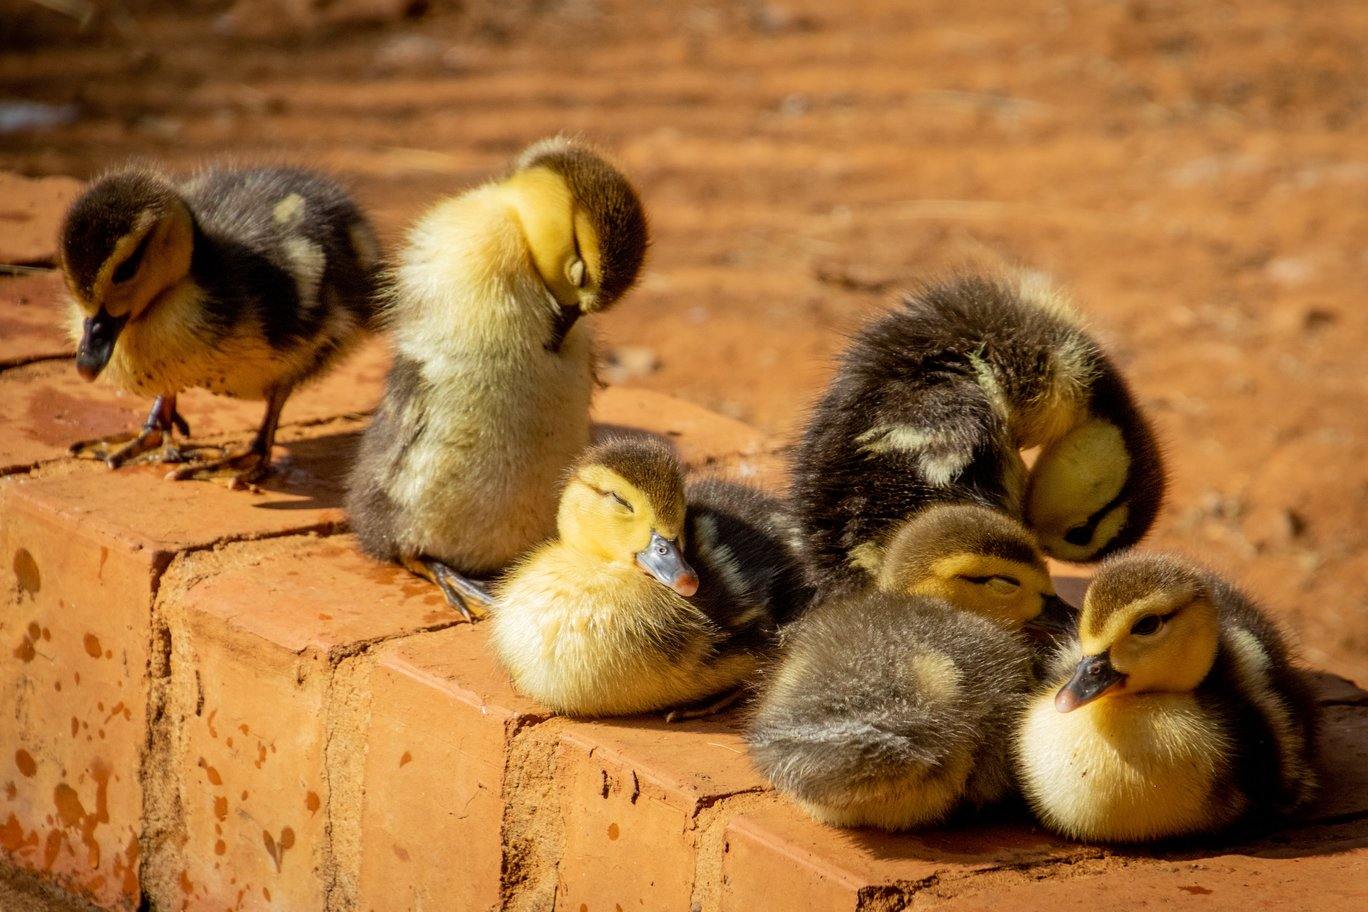
\includegraphics[width=\textwidth]{img/ducklings}
\end{center}
}
\end{document}
